\documentclass[a4paper,12pt]{article}
\usepackage{../../mypackages}
\usepackage{../../macros}

\setlength{\parindent}{0pt}


\begin{document}

\title{Feuille d'exercices - Colle Thaïs}
\author{N. Bancel}
\date{4 Décembre 2024}
\maketitle

\section{Exercice 1}

En s'inspirant de l'exercice corrigé ci-dessous, résoudre l'exercice suivant portant sur les bruleurs au bioéthanol.

\begin{figure}[H]
  \centering
  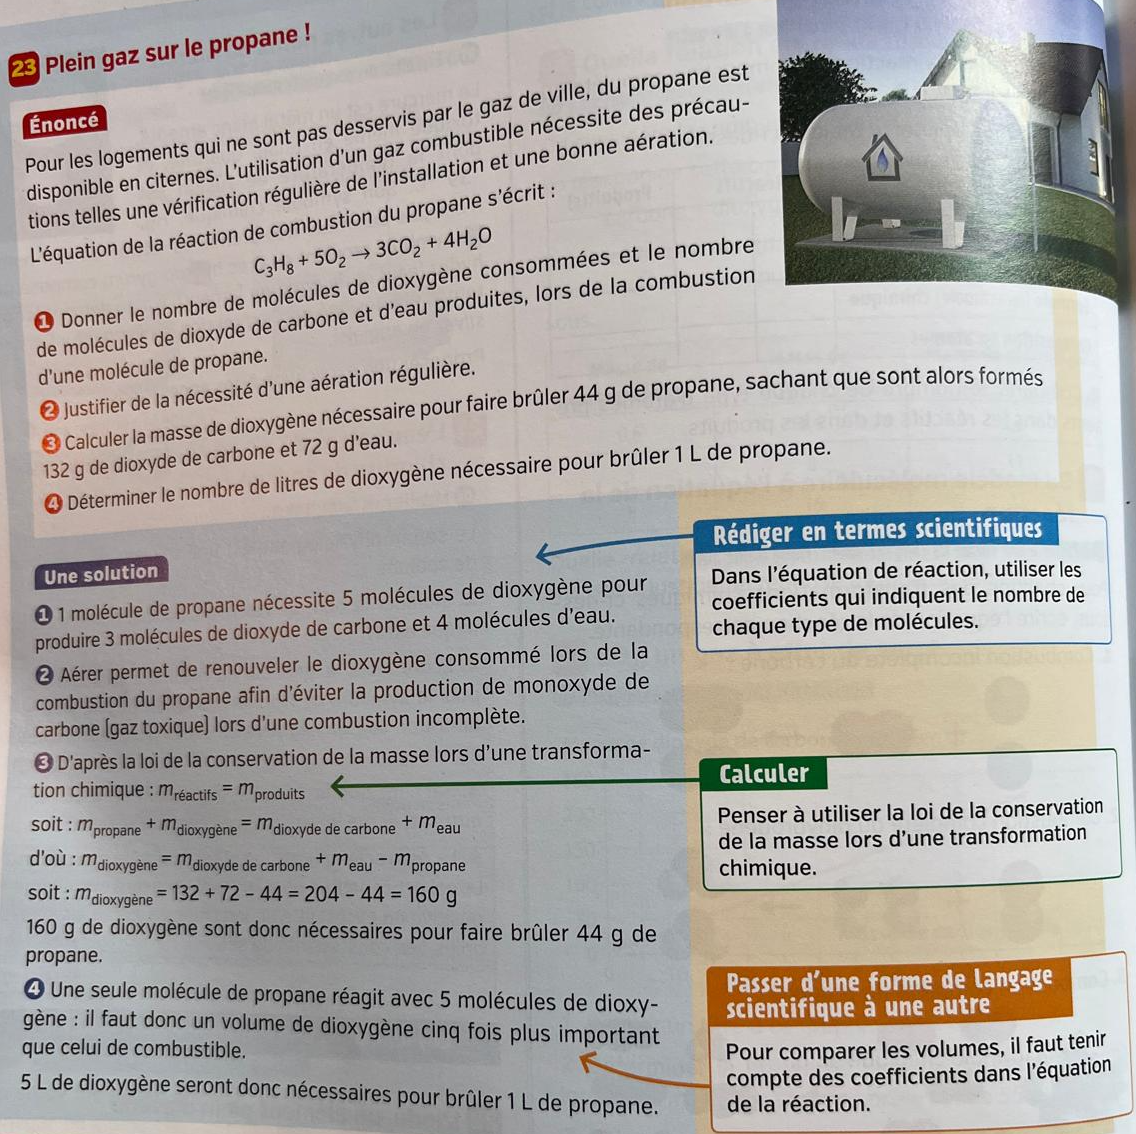
\includegraphics[width=0.8\linewidth]{img/04_03_01.png}
  \caption{\label{} Le propane}
\end{figure}

De nos jours, il existe des brûleurs au bioéthanol qui s'insèrent dans la cheminée. Le bioéthanol (alcool de betterave, constitué de molécules d'éthanol) remplace alors le bois comme combustible. L'équation de cette combusion s'écrit : 
\[
\ce{C2H6O + 3 O2 -> 2 CO2 + 3 H2O}
\]
\begin{itemize}[noitemsep]
  \item Donner le nombre de molécules de dioxygène consommées et le nombre de molécules de dioxyde de carbone et d'eau produites lors de la combustion d'une molécule d'éthanol.
  \item Calculer la masse de dioxygène nécessaire pour faire brûler 1180g d'éthanol sachant qu'il se forme 2257g de dioxyde de carbone et 1305g d'eau.
  \item Calculer le nombre de litres de dioxyde de carbone produits lorsque 6L de dioxygène sont consommés
\end{itemize}

\section{Exercice 2 - Réflexion et objectifs}

\begin{itemize}[noitemsep]
  \item Quels sont tes objectifs en Physique-Chimie pour le 2ème trimestre ?
  \item Sur quelles notions veux-tu progresser et te sens-tu moins forte ?
  \item Sur quelles notions te sens-tu à l'aise et quelles sont tes forces ?
\end{itemize}

\section{Exercice 3 - Le transport routier}

\begin{figure}[H]
  \centering
  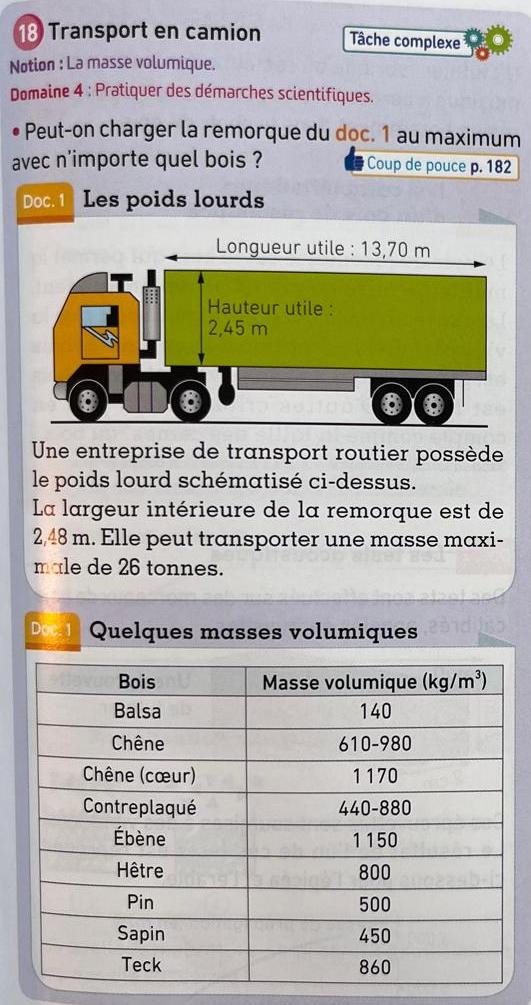
\includegraphics[width=0.3\linewidth]{img/04_03_02.jpeg}
  \caption{\label{} Exercice 3}
\end{figure}

\section{Exercice 4 - La pétanque}

\begin{figure}[H]
  \centering
  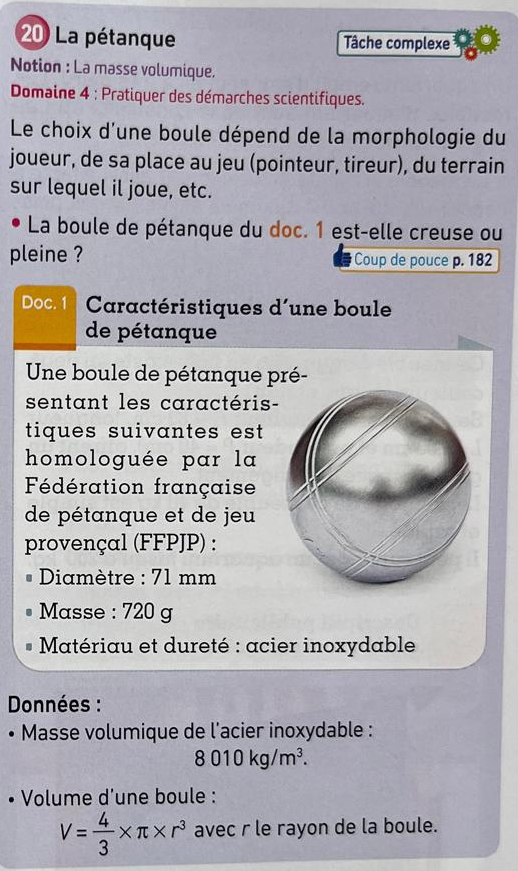
\includegraphics[width=0.3\linewidth]{img/04_03_03.png}
  \caption{\label{} Exercice 4}
\end{figure}

\end{document}
